% Intended LaTeX compiler: xelatex
\documentclass[10pt, svgnames]{beamer}
\usepackage{graphicx}
\usepackage{longtable}
\usepackage{wrapfig}
\usepackage{rotating}
\usepackage[normalem]{ulem}
\usepackage{amsmath}
\usepackage{amssymb}
\usepackage{capt-of}
\usepackage{hyperref}
\usetheme{metropolis}
\author{Sappinandana Akamphon}
\date{}
\title{Gear Design}
\subtitle{ME 310: Mechanical Design}
\usepackage{booktabs}
\usepackage[mathrm=sym]{unicode-math}
\setmathfont{Fira Math Light}
\institute{Department of Mechanical Engineering, TSE}
\AtBeginSection[]{\begin{frame}{Outline}\tableofcontents[currentsection]\end{frame}}
\hypersetup{
 pdfauthor={Sappinandana Akamphon},
 pdftitle={Gear Design},
 pdfkeywords={},
 pdfsubject={},
 pdfcreator={Emacs 30.0.50 (Org mode 9.6)}, 
 pdflang={English}}
\begin{document}

\maketitle

\section{Gear Overview}
\label{gear-overview}
\begin{frame}[label={sec:orgb5e6910}]{Why Gears?}
\begin{itemize}
\item High speed, low torque \(\rightarrow\) low speed, high torque

\item Speed: easy to get because voltage is easy

\item Torque: hard to get because it requires large current
\end{itemize}
\end{frame}

\begin{frame}[label={sec:org250578e}]{Principles of Gears}
\begin{itemize}
\item Allow positive engagement between teeth

\item High forces can be transmitted while in rolling contact

\item Do not need friction to operate \(\rightarrow\) high efficiency
\end{itemize}
\end{frame}

\begin{frame}[label={sec:org67ba456}]{Basic Law of Gearing}
\begin{itemize}
\item Point of contact between two mating gears is always the same relative
distances from the two centers.

\item Any gear tooth profiles that follow the law of gearing will result in
constant relative speed of rotation \(\rightarrow\) involute profile
\end{itemize}

\begin{center}
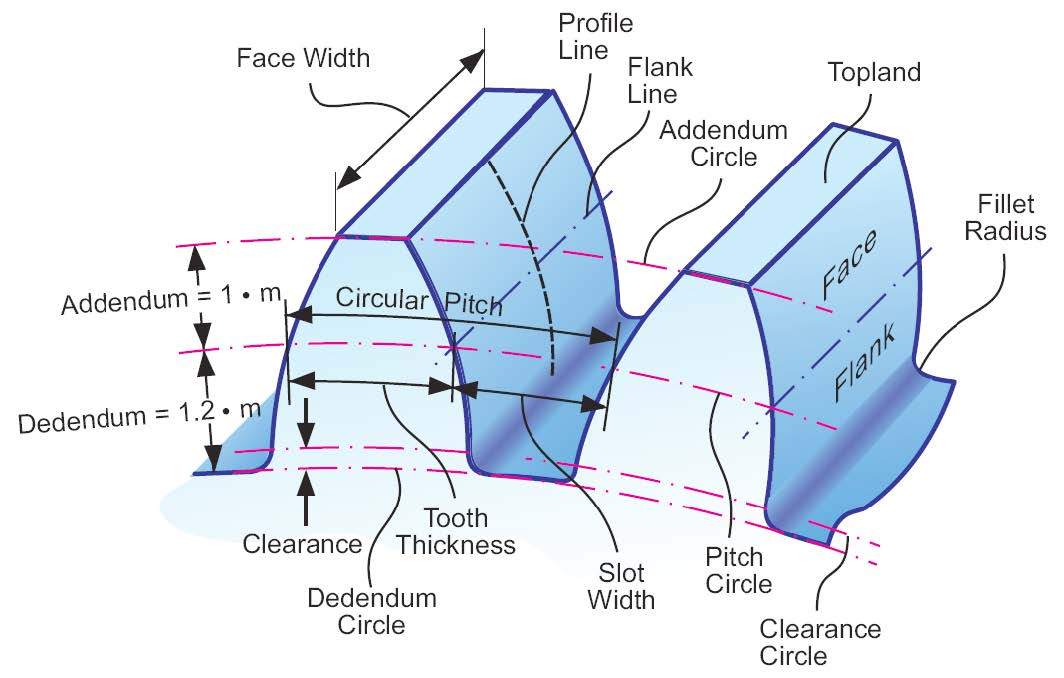
\includegraphics[width=.9\linewidth]{pictures/gear-profile.jpg}
\end{center}
\end{frame}

\begin{frame}[label={sec:orgb274fdb}]{Gear Geometry}
\begin{center}
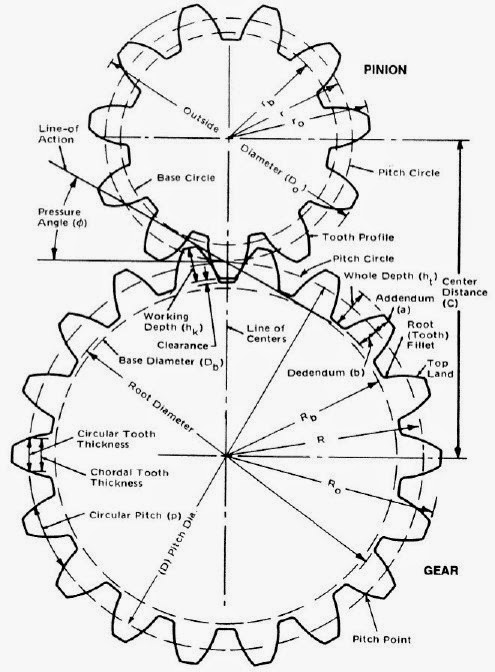
\includegraphics[width=.9\linewidth]{pictures/gear-pair.jpg}
\end{center}

Module of a Gear, \(m\)

\begin{itemize}
\item Term used to define gear tooth size

\item Defined as ratio of pitch diameter to number of teeth
\begin{align*}
  m = \frac{d}{z}
\end{align*}

\item Typical unit of mm/teeth \(\rightarrow\) must be converted to m/teeth
in most equations

\item A pair of meshing gears must have the same modules!
\end{itemize}
\end{frame}

\begin{frame}[label={sec:org4411e5e}]{Gear Types}
\begin{center}
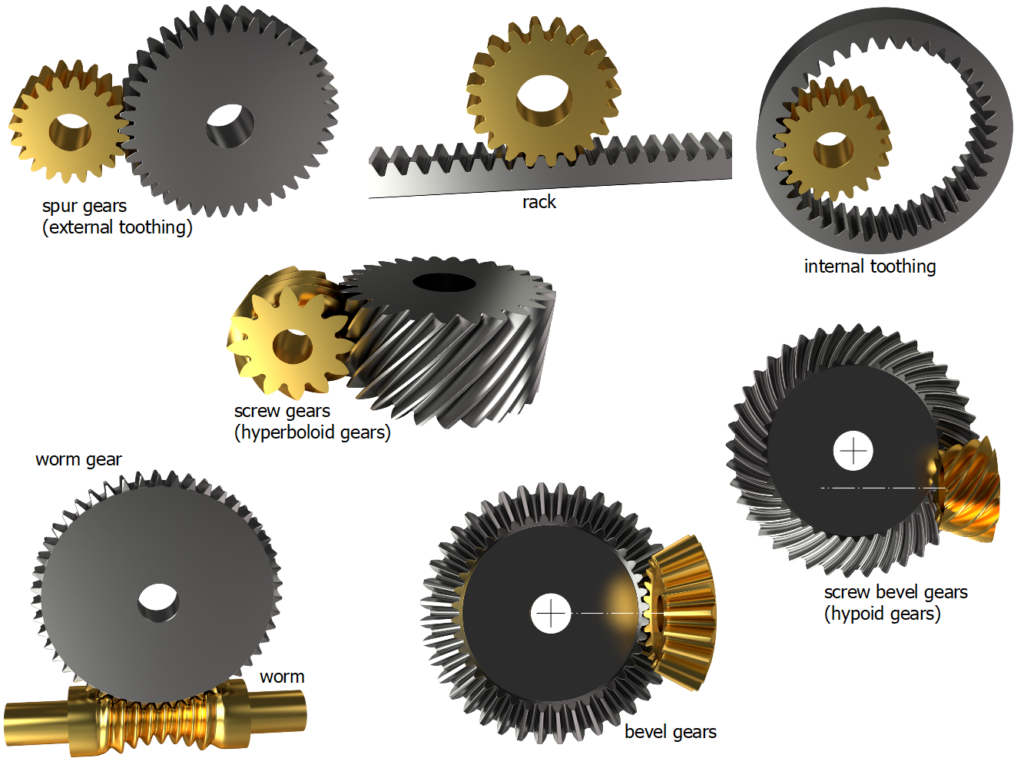
\includegraphics[width=.9\linewidth]{pictures/gear-types.png}
\end{center}
\end{frame}

\begin{frame}[label={sec:org2a29b7f}]{Gear Terminology}
\begin{description}
\item[{Pinion}] smaller of two gears, usually driving

\item[{Gear}] Larger of the two. Also called \emph{wheel}. Usually driven.
\end{description}
\end{frame}

\begin{frame}[label={sec:orgd680ec6}]{Gear Materials}
\begin{itemize}
\item Steel: medium-carbon steel + heat treatment + grinding

\item Cast iron: surface fatigue > bending fatigue

\item Nonferrous: bronzes \(\rightarrow\) corrosion + wear resistant, low
friction

\item Nonmetallic: Nylon \(\rightarrow\) low friction and weight + corrosion
resistant, but low thermal conductivity
\end{itemize}
\end{frame}

\begin{frame}[label={sec:org53ae3fd}]{Gear Efficiency}
\begin{itemize}
\item With friction, gears are 90 - 95\% efficient because of mostly rolling
contact

\begin{align*}
  T_{\text{out}} &= \frac{\eta T_{\text{in}} d_{\text{out}}}{d_{\text{in}}} \\
  \omega_{\text{out}} &= \frac{\omega_{\text{in}} d_{\text{in}}}{d_{\text{out}}} \\
  P_{\text{out}} &= T_{\text{out}} \omega_{\text{out}} \\
  RR &= \frac{\omega_{in}}{\omega_{out}} = \frac{z_{out}}{z_{in}} \approx \frac{T_{out}}{T_{in}}
\end{align*}

\item \(RR\) = gear ratio
\end{itemize}
\end{frame}

\section{Gear Trains}
\label{gear-trains}
\begin{frame}[label={sec:org873c7d3}]{Gear Trains}
\begin{columns}
\begin{column}{0.5\columnwidth}
\begin{center}
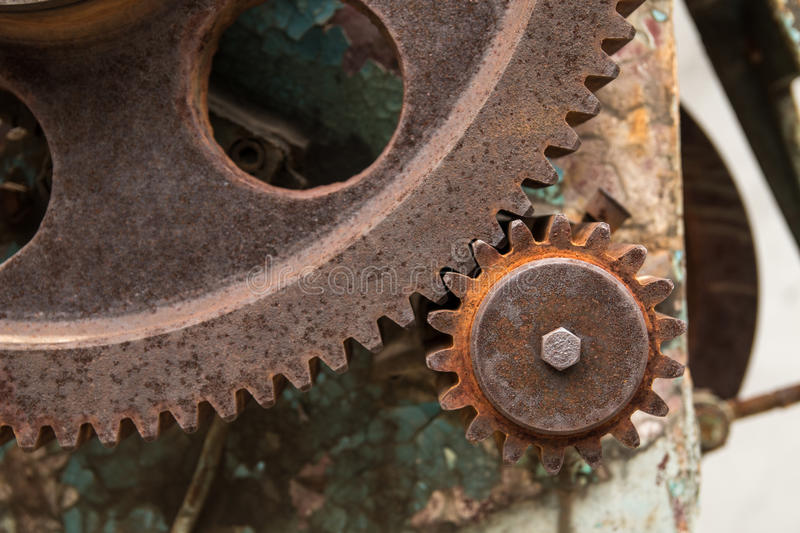
\includegraphics[width=.9\linewidth]{pictures/big-gear-small-gear.jpg}
\end{center}
\begin{center}
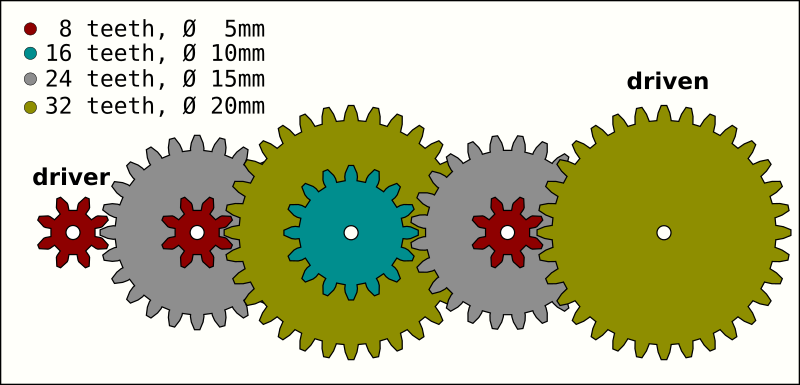
\includegraphics[width=.9\linewidth]{pictures/multi-gears.png}
\end{center}
\begin{center}
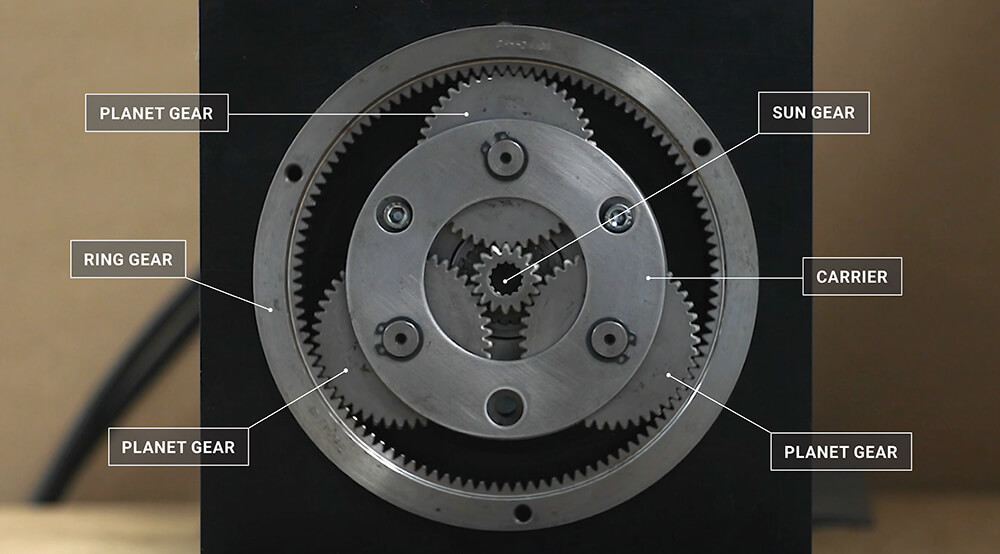
\includegraphics[width=.9\linewidth]{pictures/planetary-gear-comp.jpg}
\end{center}
\end{column}

\begin{column}{0.5\columnwidth}
When large reduction is required

\begin{itemize}
\item Large gear + small pinion: simple, but large stress and interference

\item Multiple pairs of gears and pinions: less simple, low stress, large
space

\item Planetary gears: complex, low stress, small space
\end{itemize}
\end{column}
\end{columns}
\end{frame}

\begin{frame}[label={sec:org5895274}]{Interference}
\begin{center}
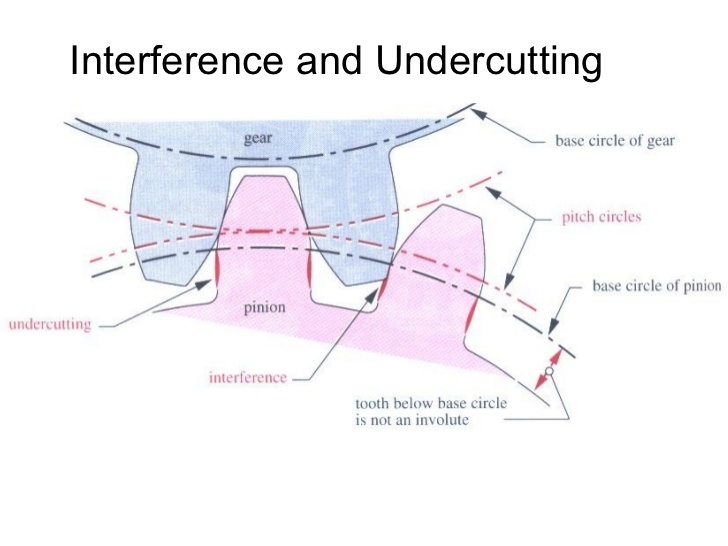
\includegraphics[width=.9\linewidth]{pictures/interference.jpg}
\end{center}
\end{frame}

\begin{frame}[label={sec:org69b6366}]{Normal Gear Trains}
\begin{center}
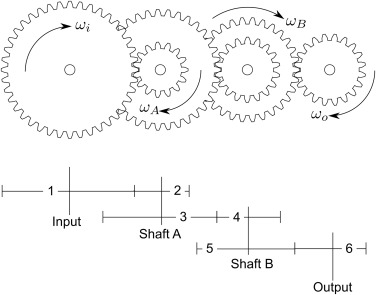
\includegraphics[width=.9\linewidth]{pictures/normal-gear-trains.jpg}
\end{center}

\begin{align*}
    RR_{total} &= RR_{1}RR_{2}\cdots
\end{align*}
\end{frame}

\begin{frame}[label={sec:org475f0bd}]{Planetary/Epicyclic Gear Train}
\begin{itemize}
\item Planetary or epicyclic gears enable a high reduction ratio in small
spaces
\end{itemize}

\begin{center}
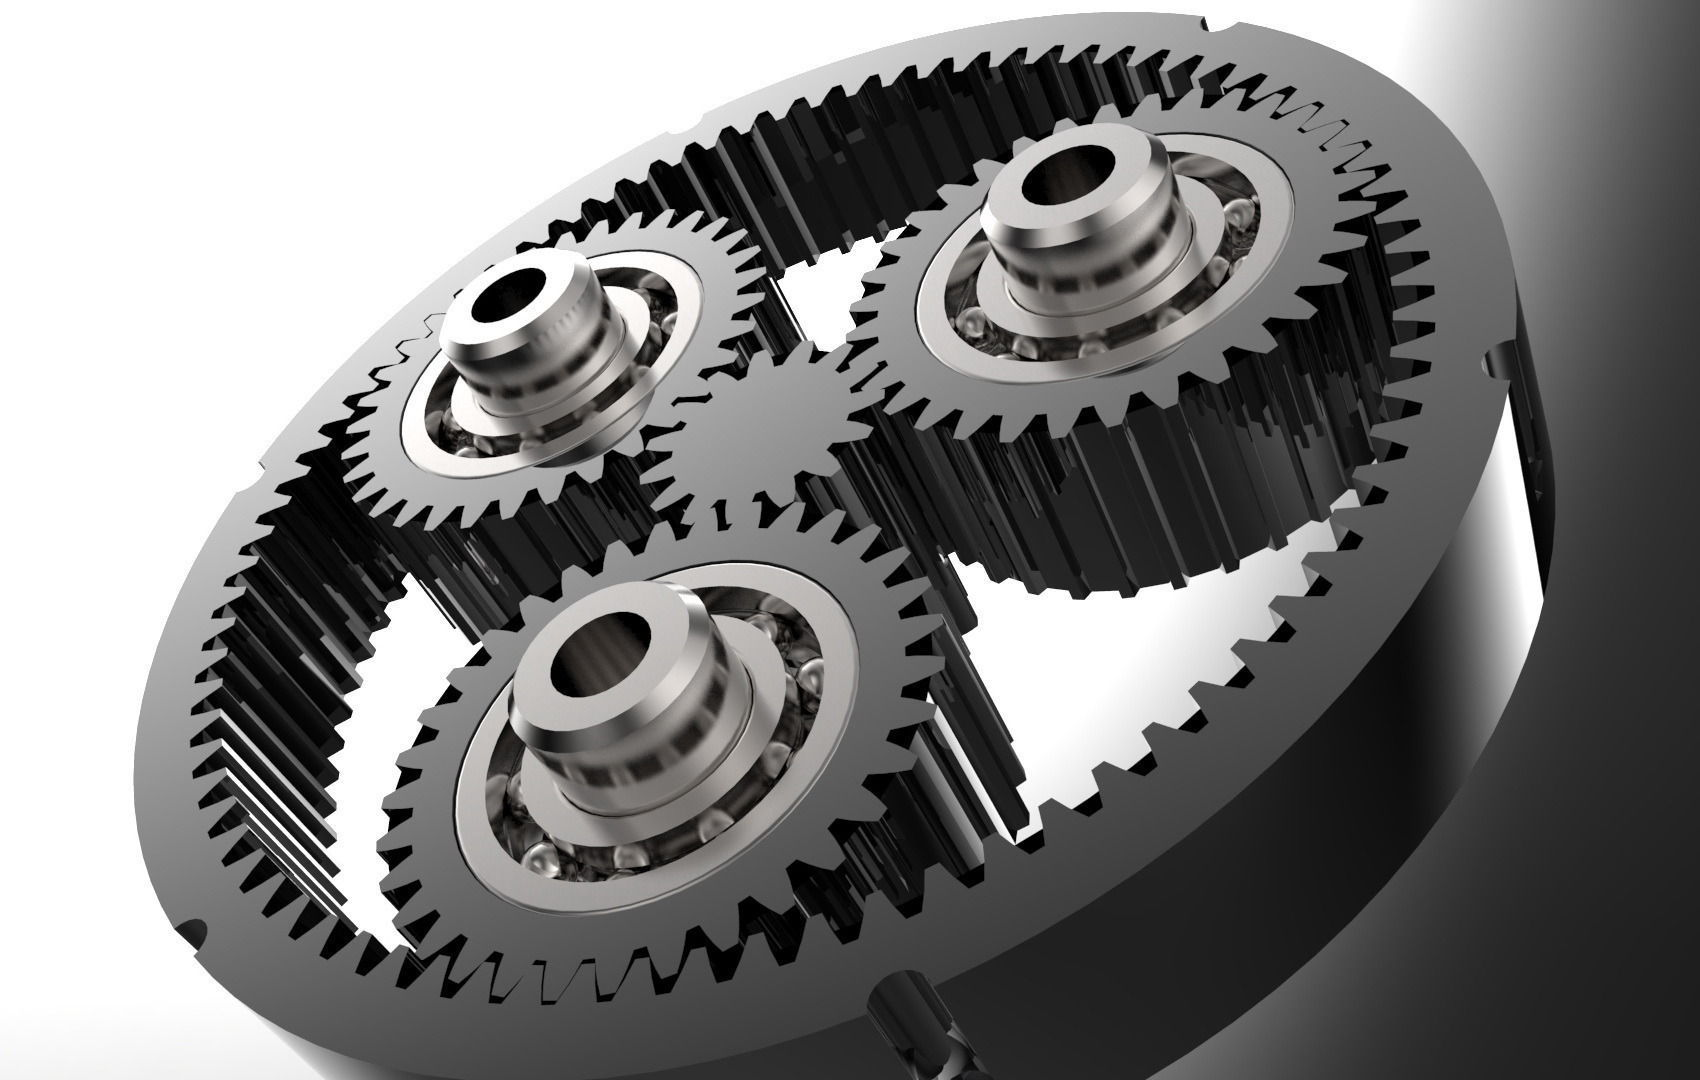
\includegraphics[width=.9\linewidth]{pictures/planetary-gearbox.jpg}
\end{center}
\end{frame}

\begin{frame}[label={sec:org7f4592e}]{Planetary Gear Components}
\begin{center}
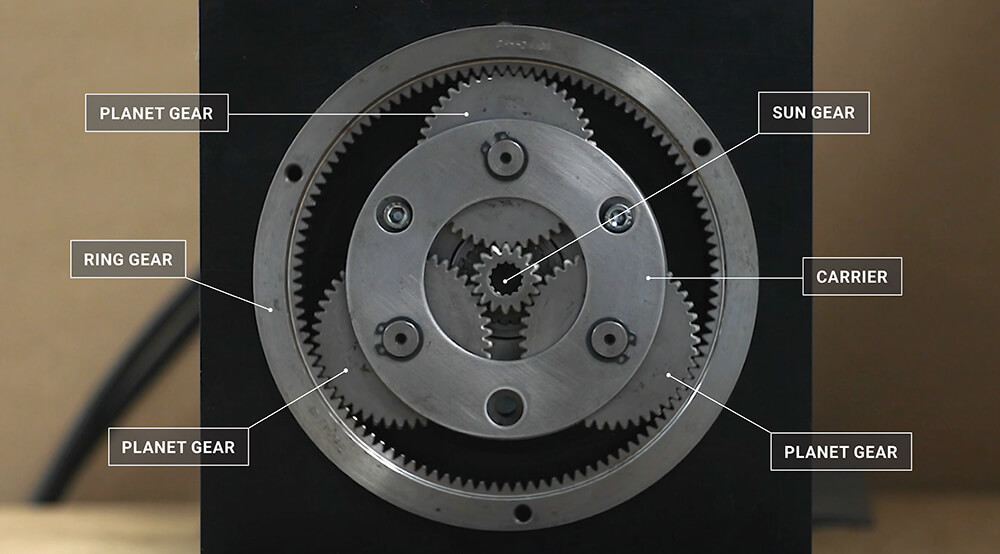
\includegraphics[width=.9\linewidth]{pictures/planetary-gear-comp.jpg}
\end{center}
\end{frame}

\begin{frame}[label={sec:orgcc2c4ea}]{Planetary Gears: Torque, Forces, and Reduction Ratios}
\begin{itemize}
\item Symmetry \(\rightarrow\) no net force on shaft

\item Multiple planet gears reduce individual torque/force

\item Any combination of fixed, input, output gears

\item 1 gear box -> multiple gear reduction ratios
\end{itemize}
\end{frame}

\begin{frame}[label={sec:orgfc9bbb0}]{Example}
\begin{columns}
\begin{column}{0.4\columnwidth}
\begin{center}
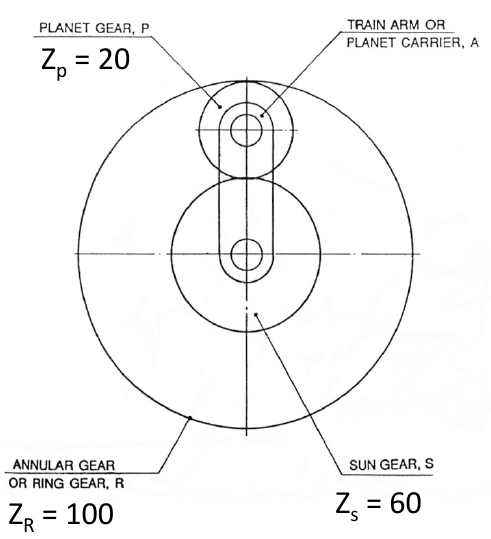
\includegraphics[width=.9\linewidth]{pictures/planet-example.png}
\end{center}
\end{column}

\begin{column}{0.6\columnwidth}
Fixed ring:

\begin{align*}
  \omega_{\text{carrier}} &= 9 \\
  \omega_{\text{planet}} &= (9) \frac{60/2 + 20/2}{20/2} = 36 \\
  \omega_{\text{sun}} &= (36) \frac{20}{30} = 24 \\
  RR &= 9/24 = 0.375
\end{align*}

\begin{center}
\begin{tabular}{llrlr}
Fixed & Input & Planet & Output & RR\\\empty
\hline
Ring & Carrier 9 & 36 & Sun 24 & 0.375\\\empty
Sun & Carrier 9 & 36 & Ring 14.4 & 0.625\\\empty
Carrier & Sun 9 & 27 & Ring 5.4 & 1.667\\\empty
\end{tabular}
\end{center}
\end{column}
\end{columns}
\end{frame}

\begin{frame}[label={sec:org9053924}]{Gear Force Analysis: The Components}
\begin{columns}
\begin{column}{0.6\columnwidth}
\begin{center}
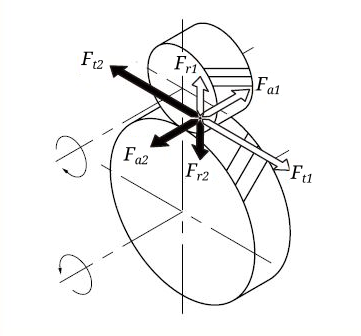
\includegraphics[width=.9\linewidth]{pictures/gear-force-analysis.png}
\end{center}
\end{column}

\begin{column}{0.6\columnwidth}
\begin{description}
\item[{\(F_{t}\)}] Tangential force (tangent to pitch circle)

\item[{\(F_{r}\)}] Radial force (passing through gear center)

\item[{\(F_{a}\)}] Axial force (parallel to axis of rotation)
\end{description}

\begin{gather*}
  \bar{F} = \bar{F_{t}} + \bar{F_{r}} + \bar{F_{a}}
\end{gather*}
\end{column}
\end{columns}
\end{frame}

\section{Spur Gears}
\label{spur-gears}
\begin{frame}[label={sec:org135a33d}]{Spur Gear Forces}
\begin{columns}
\begin{column}{0.5\columnwidth}
\begin{center}
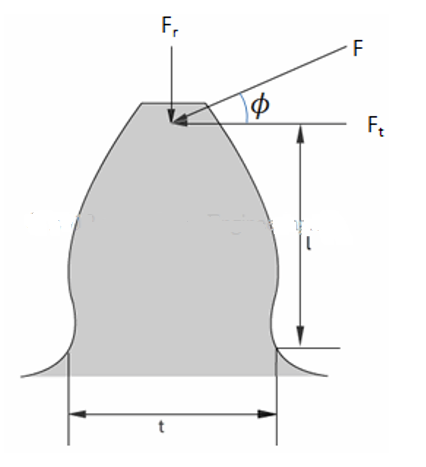
\includegraphics[width=.9\linewidth]{pictures/spur-gear-forces.png}
\end{center}
\end{column}

\begin{column}{0.5\columnwidth}
\begin{description}
\item[{\(\phi\)}] pressure angle

\item[{\(v_{t}\)}] pitch line velocity
\end{description}

\begin{align*}
  F_{t} &= \frac{\text{Power}}{v_{t}} \\
  F_{r} &= F_{t} \tan \phi \\
  F_{a} &= 0
  % F = \frac{T}{R_{\text{pitch}} \cos \theta}
\end{align*}
\end{column}
\end{columns}
\end{frame}

\begin{frame}[label={sec:org15e82c8}]{Spur Gear Stress}
\begin{itemize}
\item Bending Stress \(\rightarrow\) AGMA stress equation

\item Consider tooth as a cantilever beam
\end{itemize}

\begin{align*}
  \sigma = \frac{F_{t}}{bY_{J}m} K_{O} K_{m} K_{v}
\end{align*}

\begin{description}
\item[{\(F_{t}\)}] tangential force

\item[{\(b\)}] face width

\item[{\(Y_{J}\)}] geometry factor

\item[{\(m\)}] module

\item[{\(K_{O}\)}] overload factor

\item[{\(K_{m}\)}] mounting factor

\item[{\(K_{v}\)}] velocity factor
\end{description}
\end{frame}

\begin{frame}[label={sec:org6d941ff}]{Geometry Factor: \(Y_{J}\)}
\begin{center}
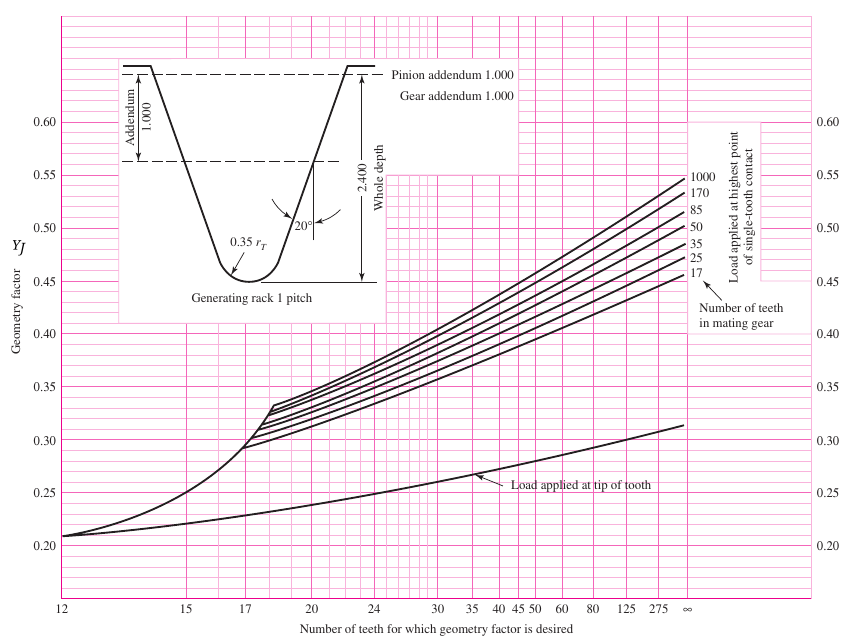
\includegraphics[width=.9\linewidth]{pictures/geometry-factor.png}
\end{center}
\end{frame}

\begin{frame}[label={sec:orgff5f00e}]{Overload Factor: \(K_{O}\)}
\small
\begin{center}
\begin{tabular}{lrrrr}
\toprule
Power source & \multicolumn{4}{c}{Driven Machine}\\% &  &  & \\\empty
\midrule
 & Uniform & Light shock & Moderate shock & Heavy shock\\\empty
Uniform & 1.00 & 1.25 & 1.50 & 1.75\\\empty
Light shock & 1.20 & 1.40 & 1.75 & 2.25\\\empty
Moderate shock & 1.30 & 1.70 & 2.00 & 2.75\\\empty
\bottomrule
\end{tabular}
\end{center}

\begin{columns}
\begin{column}{0.5\columnwidth}
Power sources

\begin{description}
\item[{Uniform}] Electric motor, constant-speed turbine

\item[{Light}] Water turbine, variable-speed drive

\item[{Moderate}] Multicylinder engine
\end{description}
\end{column}

\begin{column}{0.5\columnwidth}
Driven machine

\begin{description}
\item[{Uniform}] Continuous generator

\item[{Light}] Fans, low-speed pumps, conveyors

\item[{Moderate}] high-speed pumps, compressors, heavy conveyers

\item[{Heavy}] rock crushers, punch press drivers
\end{description}
\end{column}
\end{columns}
\end{frame}

\begin{frame}[label={sec:org8309ec5}]{Mounting Factor: \(K_{m}\)}
\begin{center}
\begin{tabular}{p{6cm}llll}
\toprule
Characteristics of Support & \multicolumn{4}{c}{Face Width (cm)} \\% &  &  & \\\empty
 & 0 to 5 & 15 & 22.5 & 40\\\empty
\midrule
Accurate mountings, small bearing clearances, precision gears & 1.3 & 1.4 & 1.5 & 1.8\\\empty
Less rigid moutings, standard gears, full face contact & 1.6 & 1.7 & 1.8 & 2.2\\\empty
Less than full face contact & \multicolumn{4}{c}{Over 2.2} \\% &  &  & \\\empty
\bottomrule
\end{tabular}
\end{center}
\end{frame}

\begin{frame}[label={sec:org0709fbc}]{Velocity Factor: \(K_{v}\)}
\begin{itemize}
\item Takes care of shock and impact loading
\end{itemize}

\begin{align*}
    K_{v} &= \left( \frac{A + \sqrt{200 v_{t}}}{A} \right)^{B} \\
    A &= 50 + 56(1 - B) \\
    B &= 0.25(12 - Q)^{2/3}
\end{align*}

\begin{description}
\item[{\(v_{t}\)}] pitch line velocity [m/s]

\item[{\(Q\)}] AGMA Quality Number
\end{description}
\end{frame}

\begin{frame}[label={sec:org1f880be}]{AGMA Recommended Quality Number: \(Q\)}
\small
\begin{center}
\begin{tabular}{lll}
\toprule
\(v_{t}\) [m/s] & \(Q\) & Applications\\\empty
\midrule
0 - 4 & 6 - 8 & Paper box making machine, cement, mill drives\\\empty
4 - 10 & 8 - 10 & Washing machine, printing press, computing mechanism\\\empty
10 - 20 & 10 - 12 & Automotive transmission, Antenna drive, propulsion drive\\\empty
\(\geqslant\) 20 & 12 - 14 & Gyroscope\\\empty
\bottomrule
\end{tabular}
\end{center}
\end{frame}

\begin{frame}[label={sec:orgc3e85c2}]{Gear Material Strength}
\begin{align*}
    S_{e}^{\prime} = S_{e}C_{L}C_{G}C_{S}k_{r}k_{t}k_{ms}
\end{align*}

\begin{description}
\item[{\(S_{e}\)}] endurance limit

\item[{\(C_{L}\)}] load factor (= 1 for bending)

\item[{\(C_{G}\)}] gradient surface = 1

\item[{\(C_{S}\)}] surface factor (= 0.75 for machined surface)

\item[{\(k_{r}\)}] reliability factor

\item[{\(k_{t}\)}] temperature factor

\item[{\(k_{ms}\)}] median-stress factor (1 for two-way bending (followers), 1.4 for one-way bending (input or output))
\end{description}
\end{frame}

\begin{frame}[label={sec:org63469b9}]{Reliability Factor: \(k_{r}\)}
\begin{center}
\begin{tabular}{lr}
\toprule
Reliability (\%) & \(k_{r}\)\\\empty
\midrule
50 & 1.000\\\empty
90 & 0.897\\\empty
99 & 0.814\\\empty
99.9 & 0.753\\\empty
99.99 & 0.702\\\empty
99.999 & 0.659\\\empty
\bottomrule
\end{tabular}
\end{center}
\end{frame}

\begin{frame}[label={sec:orgbfeb848}]{Temperature Factor: \(k_{t}\)}
\begin{align*}
    k_{t} = \left\{
    \begin{array}{cl}
      1 & T \leqslant 160 \text{ F} \\
      \hspace{5mm} \\
      \dfrac{620}{460 + T} & T > 160 \text{ F}
    \end{array}
    \right.
\end{align*}
\end{frame}

\begin{frame}[label={sec:org3ad03a2}]{General Guidelines}
\begin{enumerate}
\item \(RR \geqslant 1/6\)

\item Use multi-stage gears for larger than \(RR < 1/6\)

\item \(8m \leqslant b \leq 16m\)

\item many small teeth \(\gg\) few large teeth

\item few teeth \(\rightarrow\) small gear, but be careful about
interference

\item Avoid exact ratio \(\rightarrow\) hunting tooth
\end{enumerate}
\end{frame}

\begin{frame}[label={sec:orgcf6a984}]{Example}
A pair of spur gears with face width \(b\) = 3 cm is used in a conveyor belt drive. The input motor has \(\omega_{\max}\) of 200 rad/s. The pinion has 18 teeth. The conveyor has moderate shock and should be driven at 100 rad/s. The gears have pressure angles \(\phi\) of 20\(^{\circ}\). Both pinion and gear has \(m\) = 1 cm. Determine the maximum power that the gears can transmit continuously with 1\% chance of bending fatigue failure. Steel has \(S_{ut}\) = 400 MPa
\end{frame}

\begin{frame}[label={sec:org7dc5fab}]{Solution}
Pitch line velicity \(v_{t}\) is

\begin{align*}
   v_{t} &= \omega R_{pitch} = \frac{\omega mz}{2} \\
         &= \frac{200(0.01)(18)}{2} = 18 \text{ m/s}
\end{align*}

Determine number of teeth for mating gear (input pinion \(z_{in}\) = 18)

\begin{align*}
    \frac{z_{out}}{z_{in}} &= \frac{\omega_{in}}{\omega_{out}} \\
    z_{out} &= \frac{200(18)}{100} = 36 \text{ teeth}
\end{align*}
\end{frame}

\begin{frame}[label={sec:orge01dc27}]{Solution}
Using \(v_{t}\) = 18 m/s, select \(Q\) = 10

\begin{align*}
    B &= 0.25(12 - 10)^{2/3} = 0.397 \\
    A &= 50 + 56(1 - 0.397) = 83.77 \\
    K_{v} &= \left(\frac{83.77 + \sqrt{200(18)}}{83.77}\right)^{0.397} = 1.24
\end{align*}
\end{frame}

\begin{frame}[label={sec:org0aa2e82}]{Solution}
For other factors

\begin{description}
\item[{\(b\)}] 0.03 (face width)

\item[{\(Y_{J}\)}] 0.32 (18 pinion - 36 gear)

\item[{\(K_{O}\)}] 1.5 (input - motor, output - moderate shock conveyor)

\item[{\(K_{m}\)}] 1.6 (\(b\) = 3 cm, assuming standard gear + average
mounting)

\item[{\(K_{v}\)}] 1.24
\end{description}
\end{frame}

\begin{frame}[label={sec:org0217db7}]{Solution}
The bending fatigue stress in the gear is

\begin{align*}
    \sigma &= \frac{F_{t}}{bY_{J}m} K_{O}K_{m}K_{v} \\
           &= \frac{F_{t}}{(0.03)(0.32)(0.01)} (1.5)(1.6)(1.24) \\
           &= 31000 F_{t}
\end{align*}
\end{frame}

\begin{frame}[label={sec:orgeeff3ee}]{Solution}
Next, the material fatigue strength is

\begin{align*}
    S_{e}^{\prime} &= S_{e}C_{L}C_{G}C_{S}k_{r}k_{t}k_{ms} \\
                   &= (400 \times 10^{6}(0.5))(1)(1)(0.75)(0.814)(1)(1.4) \\
                   &= 1.71 \times 10^{8}
\end{align*}

We can then find the maximum allowable tangential force

\begin{align*}
    F_{t} &= \frac{1.71 \times 10^{8}}{31000} = 5516 \text{ N} \\
    P &= T \omega = F_{t} v_{t} = 5516 \times 18 = 9.93 \times 10^{4} \text{ W}
\end{align*}
\end{frame}

\begin{frame}[label={sec:org843dba8}]{Rack and Pinion}
\begin{columns}
\begin{column}{0.5\columnwidth}
\begin{center}
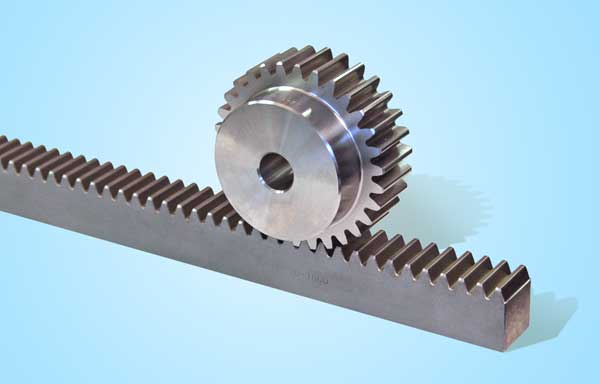
\includegraphics[width=.9\linewidth]{pictures/rack_n_pinion.jpg}
\end{center}

\begin{align*}
      F_{t} &= \frac{T}{R} \\
      F_{r} &= \frac{T \tan \phi}{R}
\end{align*}
\end{column}

\begin{column}{0.5\columnwidth}
\begin{itemize}
\item Rack = linear gear

\item Convert torque to force

\item Cheaper but less accurate than power screw

\item No mechanical advantages
\end{itemize}
\end{column}
\end{columns}
\end{frame}

\section{Helical Gears}
\label{helical-gears}
\begin{frame}[label={sec:org49be712}]{Helical Gears}
\begin{center}
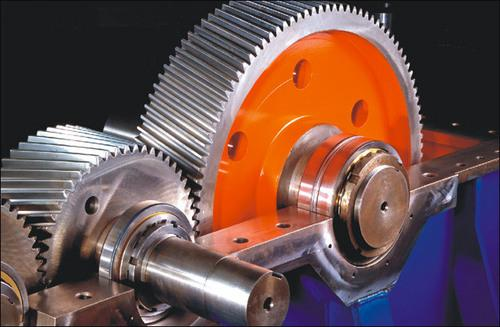
\includegraphics[width=.9\linewidth]{pictures/helical-gearbox.jpg}
\end{center}
\end{frame}

\begin{frame}[label={sec:orgaec3f0c}]{Helical Gear Force Analysis}
\begin{columns}
\begin{column}{0.6\columnwidth}
\begin{center}
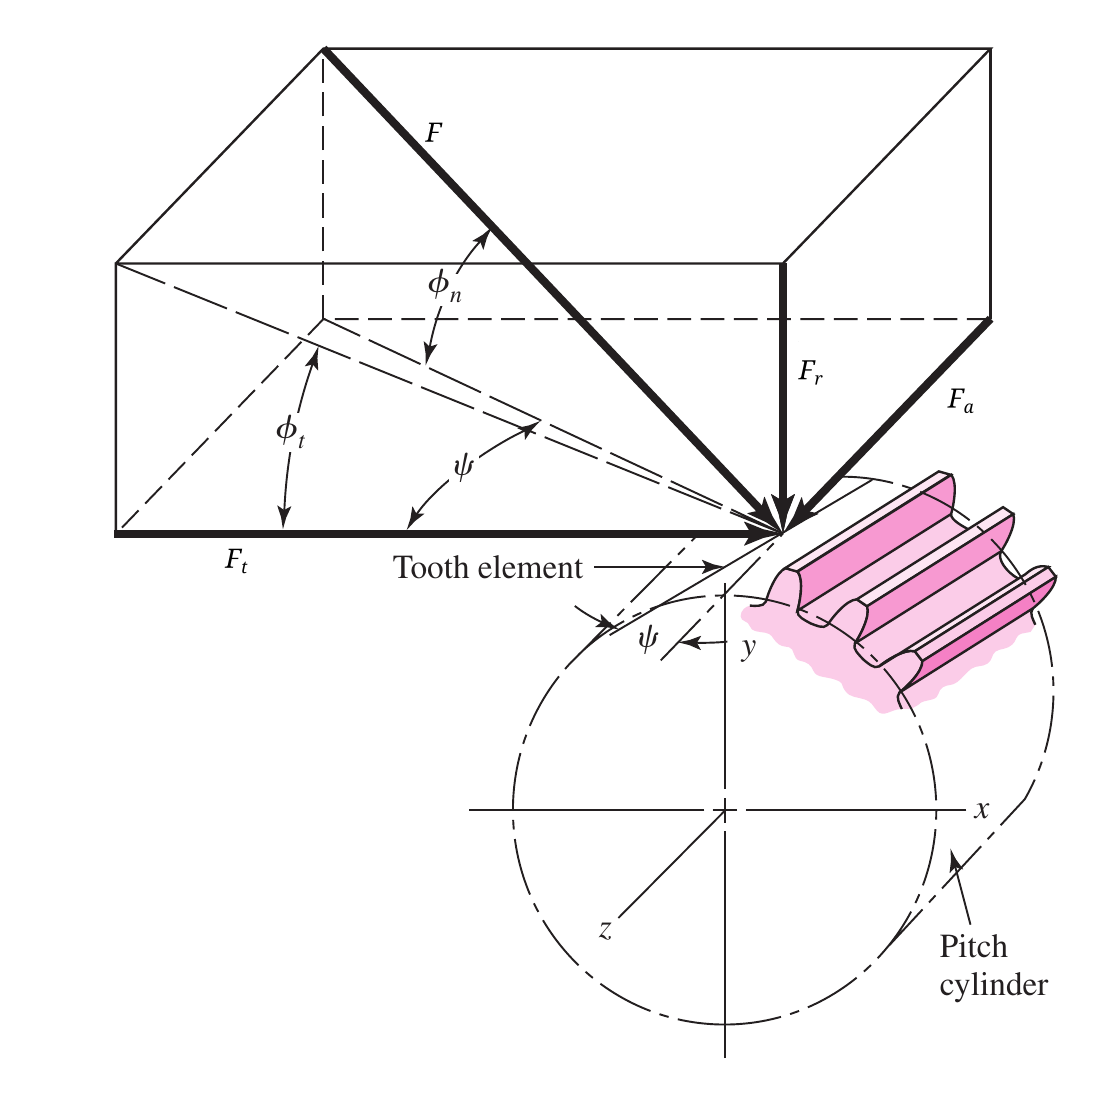
\includegraphics[width=.9\linewidth]{pictures/helical-gear-forces.png}
\end{center}
\end{column}

\begin{column}{0.5\columnwidth}
\begin{description}
\item[{\(\phi_{n}\)}] normal pressure angle

\item[{\(\phi_{t}\)}] tangential pressure angle

\item[{\(m_{n}\)}] normal module

\item[{\(m_{t}\)}] tangential module

\item[{\(\psi\)}] helix angle
\end{description}

\begin{align*}
    F_{t} &= \frac{\text{Power}}{v_{t}} \\
    F_{r} &= F_{t} \tan \phi_{t} \\
    F_{a} &= F_{t} \tan \psi \\
    \tan \phi_{n} &= \tan \phi_{t} \cos \psi \\
    m_{n} &= m_{t} \cos \psi
\end{align*}
\end{column}
\end{columns}
\end{frame}

\begin{frame}[label={sec:org58d164a}]{Why use Helical Gears?}
\begin{center}
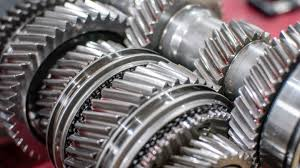
\includegraphics[width=.9\linewidth]{pictures/helical-automotive.jpg}
\end{center}

\begin{itemize}
\item Smoother operations due to gradual teeth engagement

\item Most common gears in automotive transmission
\end{itemize}
\end{frame}

\begin{frame}[label={sec:org790554e}]{Design Equations}
Same as spur gear equation with small modification

\begin{align*}
    \sigma &= \frac{F_{t}}{bY_{J}m_{t}} K_{v} K_{o} (0.93 K_{m}) \\
    S_{e}^{\prime} &= S_{e}C_{L}C_{G}C_{S}k_{r}k_{t}k_{ms}
\end{align*}

\begin{description}
\item[{0.93}] indicated helical gears less sensitivity to mounting factor

\item[{\(Y_{J}\)}] needs small modification for helical teeth
\end{description}
\end{frame}

\begin{frame}[label={sec:orga37e3b2}]{Geometry Factor: \(Y_{J}\)}
\begin{center}
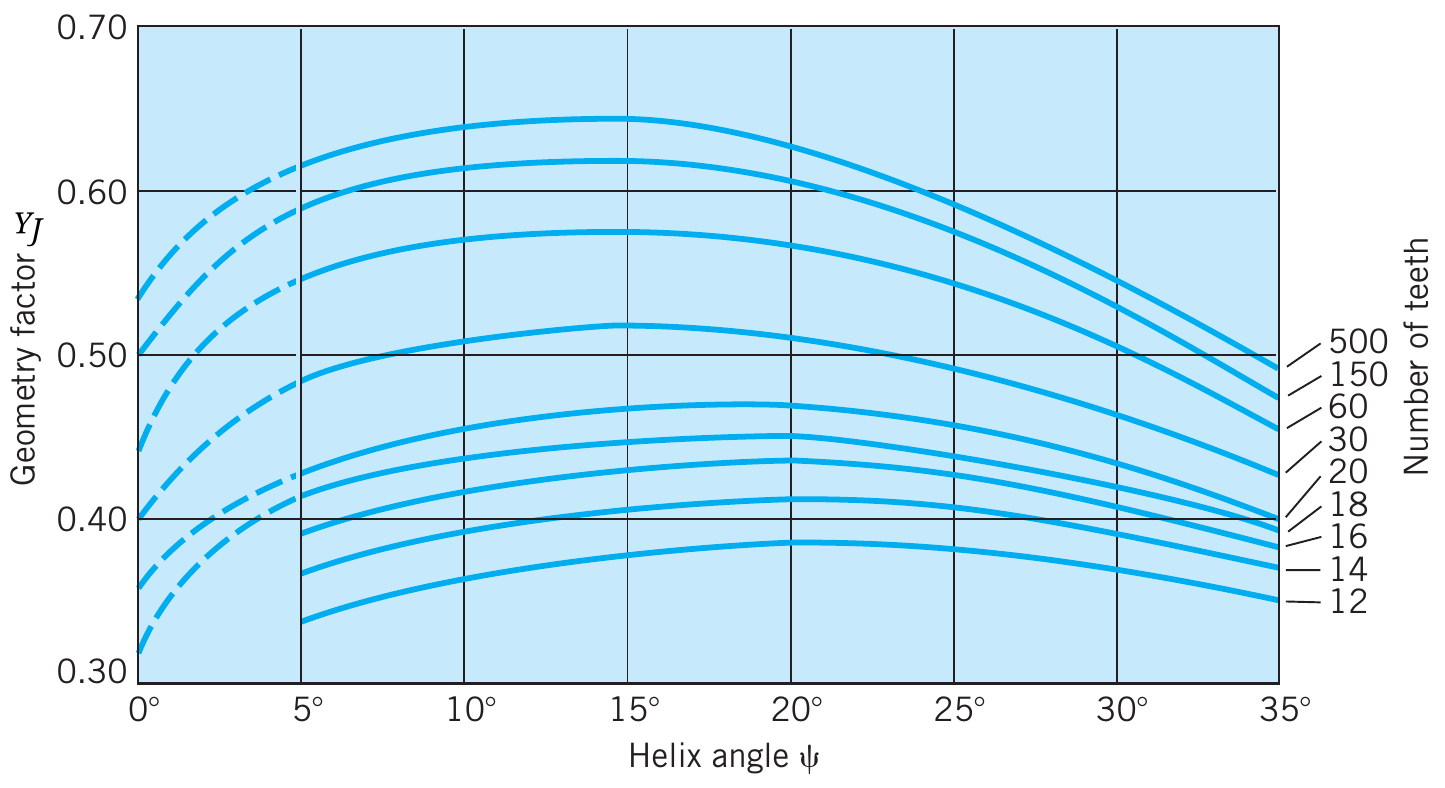
\includegraphics[width=.9\linewidth]{pictures/geometry-factor-helical.png}
\end{center}
\end{frame}

\begin{frame}[label={sec:org6c5dcf6}]{Geometry Factor Multiplier: \(Y_{J}\)}
\begin{center}
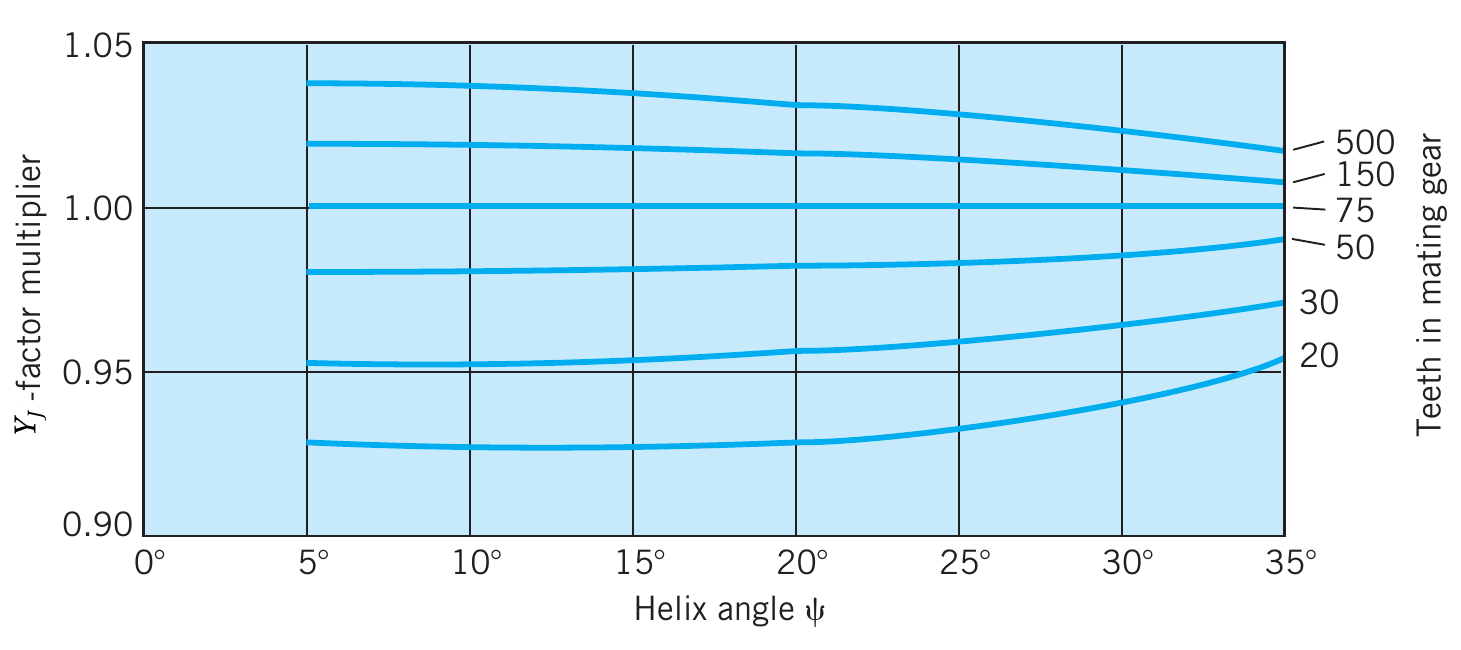
\includegraphics[width=.9\linewidth]{pictures/geometry-factor-multiplier-helical.png}
\end{center}
\end{frame}

\begin{frame}[label={sec:orgf1c0ddd}]{Example: Meshing Helical Gears}
A pair of meshing helical gears is connected at the input side to a 0.5-hp motor at 1800 rpm and to an output shaft at 600 rpm. The input gear has 18 teeth, \(\phi_{n}\) = 20\(^{\circ}\), \(m_{n}\) = 0.00173, \(\psi\) = 30\(^{\circ}\), \(b\) = 2 cm. From the given information, determine the pitch line velocity \(v_{t}\), gear tooth forces \(F_{t}, F_{r}, \text{ and } F_{a}\), and bending stress \(\sigma\).
\end{frame}

\begin{frame}[label={sec:org8f2732a}]{Solution: Meshing Helical Gears}
Calculate tangential module from normal module, then pitch diameter and tangential velocity.

\begin{align*}
    m_{t} &= \frac{m_{n}}{\cos 30^{\circ}} = \frac{0.00173}{\cos 30^{\circ}} = 0.002 \\
    d &= mz = 0.002(18) = 0.036 \text{ m} \\
    v_{t} &= \omega \frac{d}{2}  = (1800) \frac{2\pi}{60} \frac{0.036}{2} = 3.4 \text{ m/s}
\end{align*}
\end{frame}

\begin{frame}[label={sec:orgc3e9518}]{Solution: Meshing Helical Gears}
Transmitted power only depends on tangential force, after which we can calculate axial and radial forces.

\begin{align*}
    F_{t} &= \frac{\text{Power}}{v_{t}} = \frac{0.5(746)}{3.4} = 104 \text{ N} \\
    \tan \phi_{t} &= \frac{\tan \phi_{n}}{\cos \psi} = \frac{\tan 20^{\circ}}{\cos 30^{\circ}} = 0.42 \\
    \phi_{t} &= 22.8^{\circ} \\
    F_{r} &= F_{t}\tan \phi_{t} = 104 \tan 22.8^{\circ} = 43.7 \text{ N} \\
    F_{a} &= F_{t} \tan \psi = 104 \tan 30^{\circ} = 60 \text{ N}
\end{align*}
\end{frame}

\begin{frame}[label={sec:orge6e6c85}]{Solution: Meshing Helical Gears}
\begin{align*}
    \sigma &= \frac{F_{t}}{bY_{J}m_{t}}K_{v}K_{o}(0.93K_{m})
\end{align*}

\(b\) = 0.02 m

For 18-teeth to 54-teeth mesh, \(Y_{J}\) = 0.99(0.42) = 0.416

Uniform-uniform input-output, \(K_{o}\) = 1
\end{frame}

\begin{frame}[label={sec:orgdd7ebc8}]{Solution: Meshing Helical Gears}
For \(K_{v}\), since \(v_{t}\) = 3.57 m/s, let \(Q\) = 6.

\begin{align*}
     B &= 0.25(12 - 6)^{2/3} = 0.825 \\
     A &= 50 + 56(1 - 0.825) = 59.8 \\
     K_{v} &= \left( \frac{59.8 + \sqrt{200v_{t}}}{59.8} \right)^{0.825} = 1.36
\end{align*}

For \(K_{m}\), nothing specific about gears or mounting, let's go with the middle case for \(b\) = 2 cm. \(K_{m}\) = 1.6
\end{frame}

\begin{frame}[label={sec:org34cd9ff}]{Solution: Meshing Helical Gears}
We can finally calculate \(\sigma\)

\begin{align*}
    \sigma &= \frac{F_{t}}{bY_{J}m_{t}}K_{v}K_{o}(0.93K_{m}) \\
           &= \frac{104}{(0.02)(0.416)(0.002)}(1.36)(1)((0.93)1.6) \\
           &= 1.26 \times 10^{7} = 12.6 \text{ MPa}
\end{align*}
\end{frame}

\section{Bevel Gears}
\label{bevel-gears}
\begin{frame}[label={sec:org0de6cf6}]{Bevel Gears}
\begin{center}
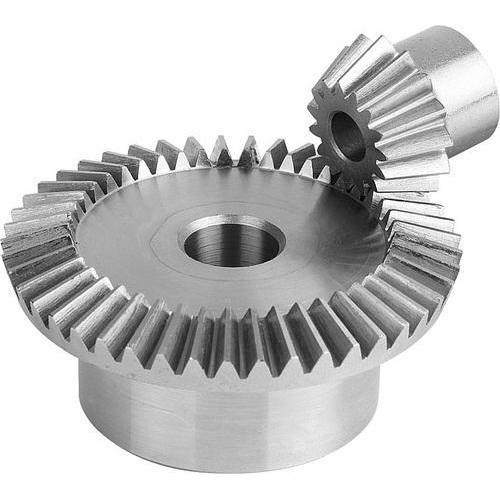
\includegraphics[height=0.8\textheight]{pictures/bevel-pair.png}
\end{center}
\end{frame}

\begin{frame}[label={sec:org95a32c9}]{Bevel Gear Geometry}
\begin{center}
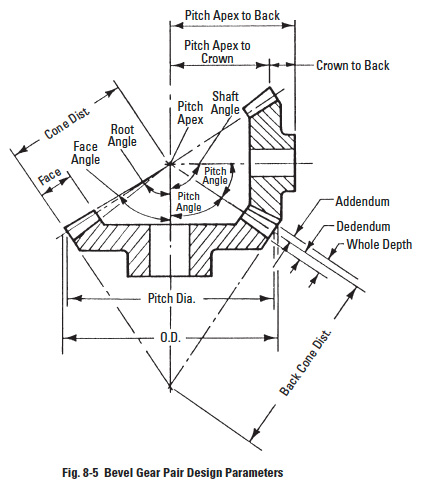
\includegraphics[width=.9\linewidth]{pictures/bevel-geometry2.jpg}
\end{center}
\end{frame}

\begin{frame}[label={sec:org0511277}]{Bevel Gears}
\begin{columns}
\begin{column}{0.5\columnwidth}
\begin{center}
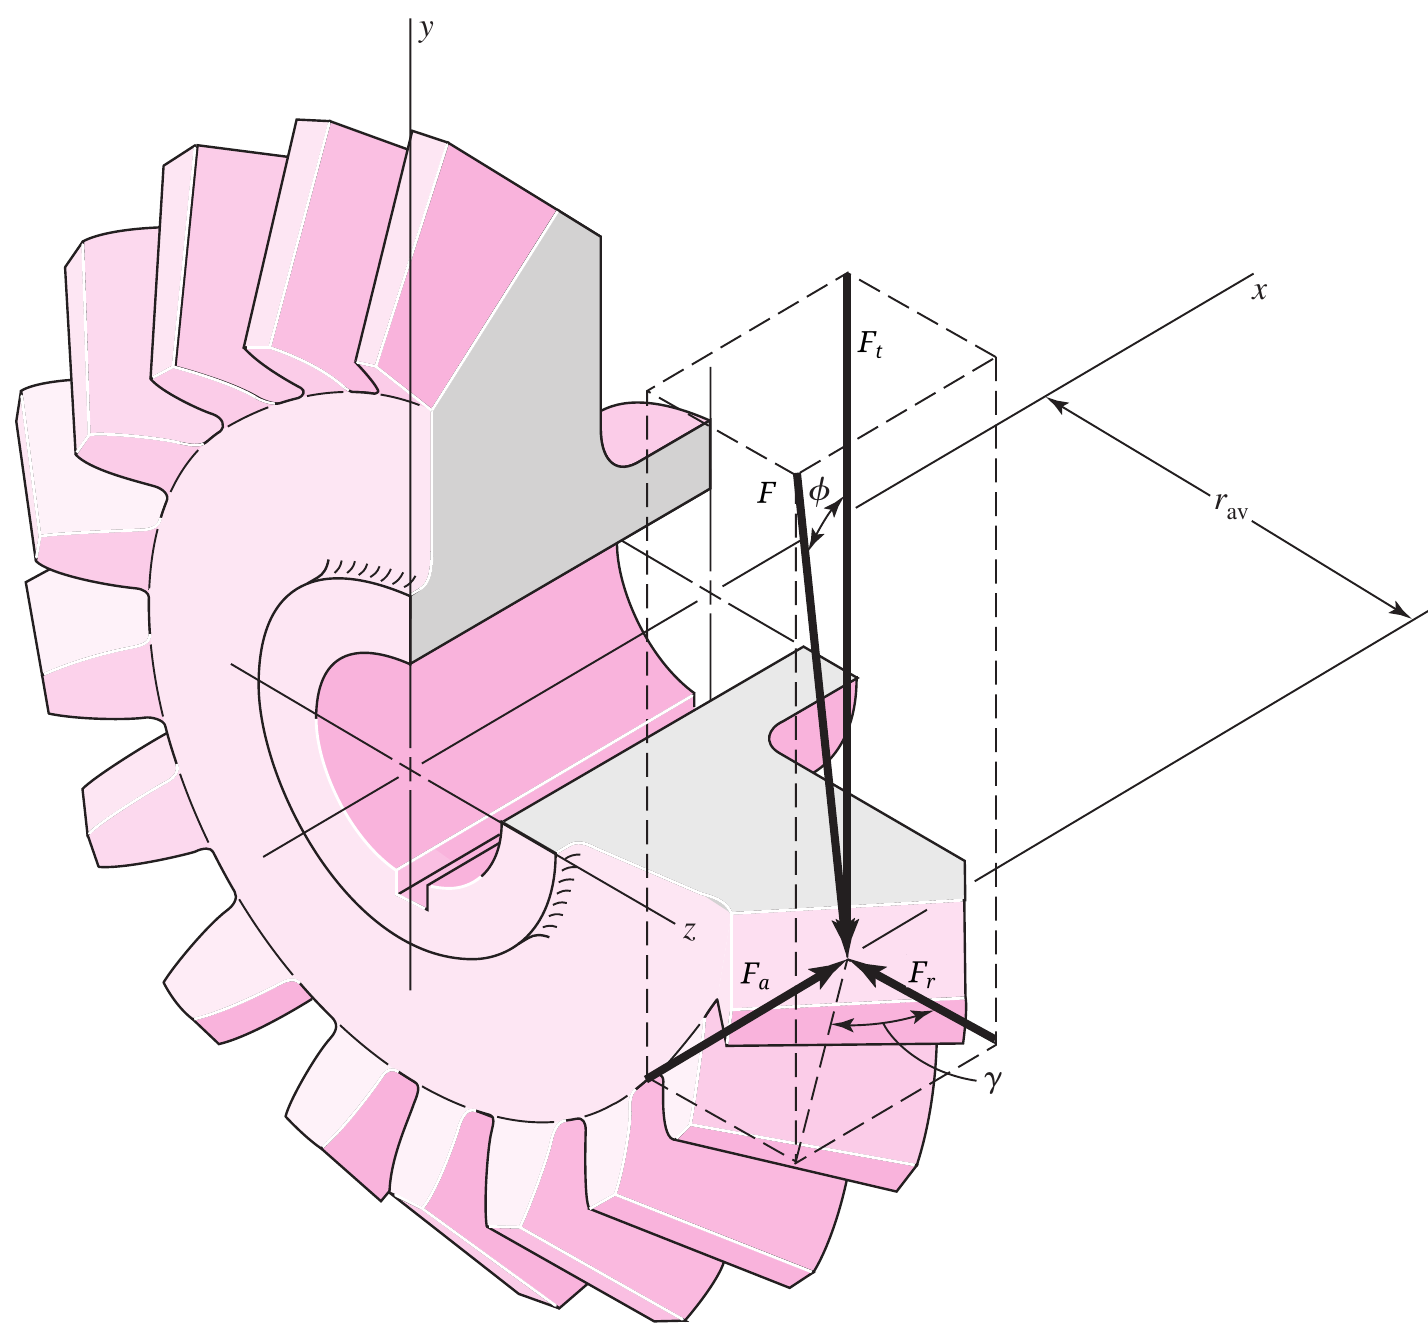
\includegraphics[width=1.2\textwidth]{pictures/bevel-gear-forces.png}
\end{center}
\end{column}

\begin{column}{0.5\columnwidth}
\begin{description}
\item[{\(\gamma\)}] pitch angle

\item[{\(\phi\)}] pressure angle

\begin{align*}
  d_{av} &= d - b \sin \gamma \\
  v_{av} &= \omega \frac{d_{av}}{2} \\
  F_{t} &= \frac{\text{Power}}{v_{av}} \\
  F_{a} &= F_{t} \tan \phi \sin \gamma \\
  F_{r} &= F_{t} \tan \phi \cos \gamma
\end{align*}
\end{description}
\end{column}
\end{columns}
\end{frame}

\begin{frame}[label={sec:org762cada}]{Design Equations}
Same as spur gear equation with small modification

\begin{align*}
    \sigma &= \frac{F_{t}}{bY_{J}m} K_{v} K_{o} K_{m} \\
    S_{e}^{\prime} &= S_{e}C_{L}C_{G}C_{S}k_{r}k_{t}k_{ms}
\end{align*}
\end{frame}

\begin{frame}[label={sec:org678f012}]{Geometry Factor: \(Y_{J}\)}
\begin{center}
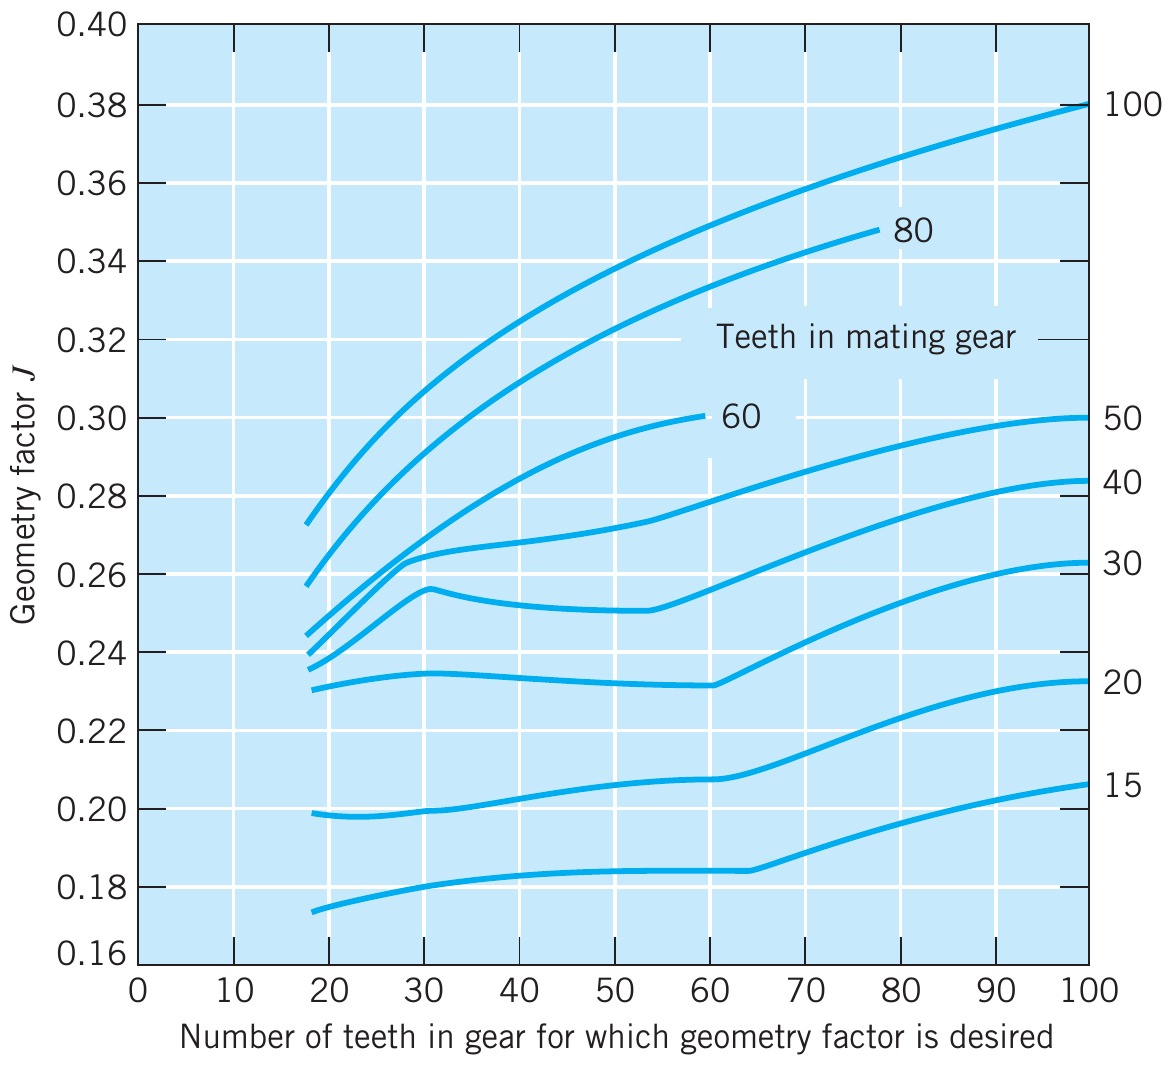
\includegraphics[width=.9\linewidth]{pictures/geometry-factor-bevel.png}
\end{center}
\end{frame}

\begin{frame}[label={sec:org1304235}]{Mounting Factor: \(K_{m}\)}
\begin{center}
\begin{tabular}{lp{4cm}l}
\toprule
Mounting type &  & Mounting Rigidity\\\empty
\midrule
Both straddle-mounted & 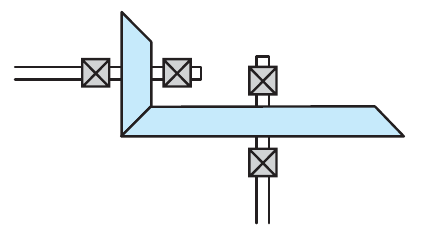
\includegraphics[width=0.3\textwidth]{pictures/both-straddle} & 1.0 to 1.25\\\empty
straddle-overhung & 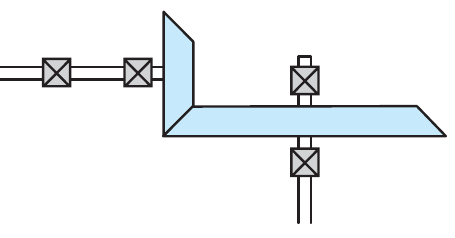
\includegraphics[width=0.3\textwidth]{pictures/straddle-overhung} & 1.1 to 1.4\\\empty
Both overhung & 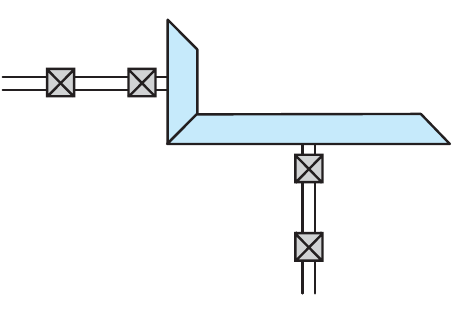
\includegraphics[width=0.3\textwidth]{pictures/both-overhung} & 1.25 to 1.5\\\empty
\bottomrule
\end{tabular}
\end{center}
\end{frame}

\begin{frame}[label={sec:orgc065327}]{Example: Bevel Gearset Design}
Identical bevel gears has a module of 0.005 m/teeth, 25 teeth, 2-cm face width, and a \(20^{\circ}\) normal pressure angle. The gear quality is \(Q = 7\). Both requires overhung mounting. The gears are made of ductile iron whose \(S_{e}\) = 95 MPa. Determine the power rating of the gearset at 600 rpm.
\end{frame}

\begin{frame}[label={sec:orgcebb517}]{Solution: Bevel Gearset Design}
For the stress side,
\begin{align*}
    d_{av} &= mz = 0.125 \text{ m} \\
    v_{t} &= \omega \frac{d_{av}}{2} = 600 \frac{2\pi}{60} \frac{0.125}{2} = 3.93 \text{ m/s}
\end{align*}

For uniform-uniform loading, \(K_{o} = 1\)
\begin{align*}
    B &= 0.25(12 - 7)^{2/3} = 0.731 \\
    A &= 50 + 56(1 - 0.731) = 65 \\
    K_{v} &= \left( \frac{65 + \sqrt{200(3.93)}}{65} \right)^{0.731} = 1.3
\end{align*}

For both-overhung mounting, \(K_{m} = 1.5\)

For 25-teeth pair, \(Y_{J}\) = 0.22
\end{frame}

\begin{frame}[label={sec:org8e3ebd1}]{Solution: Bevel Gearset Design}
Now, onto the strength side,

\begin{description}
\item[{\(C_L\)}] = 1 for bending

\item[{\(C_{s}\)}] = 0.75 for machined surface

\item[{\(C_{G}\)}] = 1
\end{description}

No requirement on the reliablility. Let's be generous, give it 90\% so
that \(k_{r} = 0.897\).

For normal operating temperature, \(k_{t}\) = 1.

For one-way bending, \(k_{ms}\) = 1.4.
\end{frame}

\begin{frame}[label={sec:orge44c906}]{Solution: Bevel Gearset Design}
Set the two sides equal (\(N_{s}\) = 1), we have

\begin{gather*}
    \frac{F_{t}}{(0.02)(0.22)(0.005)}(1.3)(1)(1.5) = 95 \times 10^{6} (1)(1)(0.75)(0.897)(1)(1.4) \\
    F_{t} = 1009 \text{ N} \\
    \text{Power} = F_{t}v_{t} = 1009(3.93) = 3965 \text{ W} = 5.31 \text{ hp}
\end{gather*}
\end{frame}

\section{Worms and Worm Gears}
\label{worms-and-worm-gears}
\begin{frame}[label={sec:org785c5e6}]{Worm Force Analysis}
\begin{center}
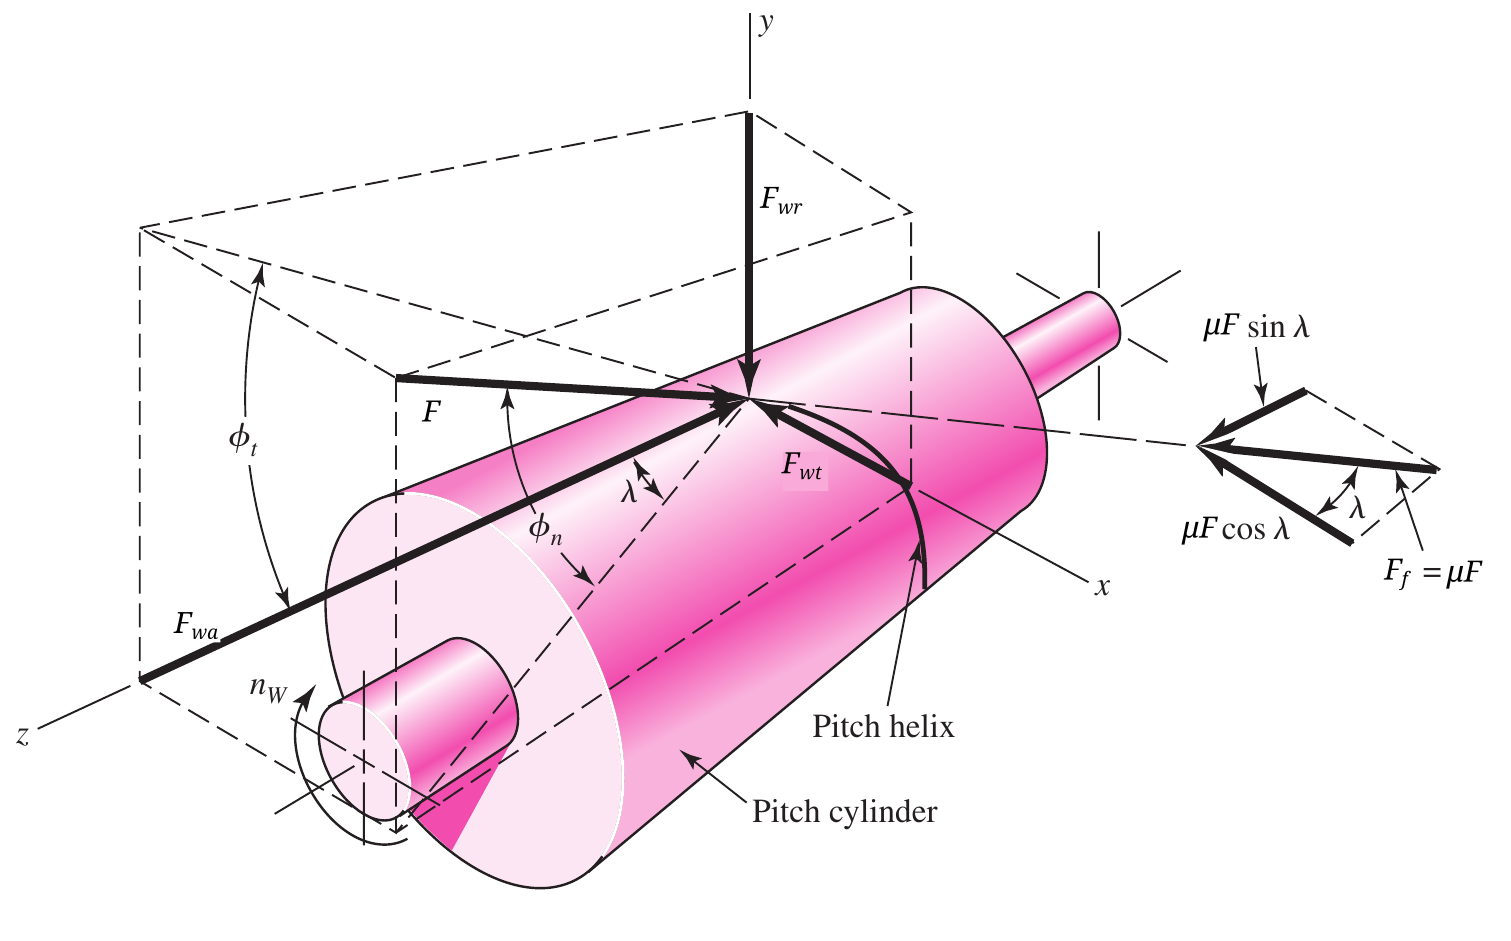
\includegraphics[width=0.7\textwidth]{pictures/worm-gear-forces.png}
\end{center}

\begin{itemize}
\item With friction \(F_{f} = \mu F\), \(\lambda\) = lead angle,
\(\phi_{n}\) = normal pressure angle
\begin{align*}
  F_{wt} &= F \cos \phi_{n} \sin \lambda + \mu F \cos \lambda = F_{ga} \\
  F_{wr} &= F \sin \phi_{n} = F_{gr} \\
  F_{wa} &= F \cos \phi_{n} \cos \lambda - \mu F \sin \lambda = F_{gt}
\end{align*}
\end{itemize}
\end{frame}

\begin{frame}[label={sec:org890e4a8}]{Worm Force Analysis II}
\begin{figure}[htbp]
  \centering
  \begin{tikzpicture}[>=latex]
    \node{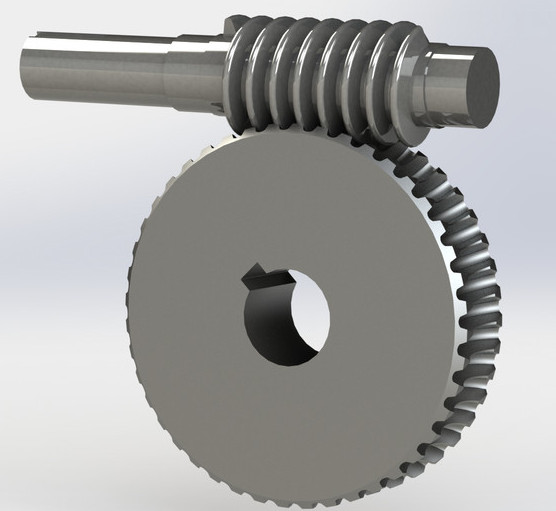
\includegraphics[height=0.9\textheight]{pictures/gear-worm-force-analysis}};
    \node at (0.6,2.0)[circle, fill=Black, draw, minimum height=1mm, inner sep=0](contact){};
    \draw [Blue, ->, very thick] (contact.center) --++ (30:2) node[below right]{$F_{ga}$};
    \draw [Blue, ->, very thick] (contact.center) --++ (270:2) node[right]{$F_{gr}$};
    \draw [Blue, ->, very thick] (contact.center) --++ (170:2) node[left]{$F_{gt}$};
    \draw [Black, ->, very thick] (contact.center) --++ (210:2) node[below right]{$F_{wt}$};
    \draw [Black, ->, very thick] (contact.center) --++ (90:2) node[right]{$F_{wr}$};
    \draw [Black, ->, very thick] (contact.center) --++ (-10:2) node[right]{$F_{wa}$};
  \end{tikzpicture}
\end{figure}
\end{frame}

\begin{frame}[label={sec:org66c4dc4}]{Worm Efficiency}
\begin{itemize}
\item Worm and worm gear velocities can be related by
\end{itemize}

\begin{align*}
    \frac{v_{g}}{v_{w}} &= \tan \lambda \\
    v_{s} &= \sqrt{v_{w}^{2} + v_{g}^{2}} = v_{w} \sqrt{1 + \tan^{2} \lambda}
\end{align*}

\begin{itemize}
\item Efficiency \(\eta\) is
\end{itemize}

\begin{align*}
    \eta &= \frac{F_{gt}v_{g}}{F_{wt}v_{w}} \\
         &= \frac{\cos \phi_{n} \cos \lambda - \mu \sin \lambda}{\cos \phi_{n} \sin \lambda + \mu \cos \lambda} \tan \lambda \\
         &= \frac{\cos \phi_{n} - \mu \tan \lambda}{\cos \phi_{n} + \mu \cot \lambda}
\end{align*}
\end{frame}

\begin{frame}[label={sec:org6955115}]{Self-Locking}
\begin{itemize}
\item Thread will lock itself (not backdrivable) when \(F_{wt} \leqslant 0\)
\begin{align*}
  F_{wt} &= F \cos \phi_{n} \sin \lambda - \mu F \cos \lambda \leqslant 0 \\
  \mu &\geqslant \cos \phi_{n} \tan \lambda
\end{align*}

\item Note that when gear drives worm, friction direction is reversed (hence
the negative sign)

\item Desirable in cases where auto-braking is needed

\item In systems with large inertia, sudden stop can break the worm tooth \(\rightarrow\) alternative brake mechanism is needd
\end{itemize}
\end{frame}

\begin{frame}[label={sec:orga25b089}]{Worm Gear Design Equations}
Worm gears have higher stresses than worm, so our main concern is designing the gear.

\begin{align*}
    F_{gt, allow} = \frac{C_{s}d^{0.8}bC_{m}C_{v}}{75.948}
\end{align*}

\begin{description}
\item[{\(F_{gt, allow}\)}] allowable gear force [N]

\item[{\(C_s\)}] material factor

\item[{\(d\)}] gear diameter [mm]

\item[{\(b\)}] effective face width (actual width but less than
0.67\(d_{w}\)) [mm]

\item[{\(C_{m}\)}] ratio correction factor

\item[{\(C_{v}\)}] velocity factor
\end{description}
\end{frame}

\begin{frame}[label={sec:orgdb0d858}]{\(C_{s}\): Material factor}
For center distance \(C < 76.2\) mm
\begin{align*}
    C_{s} = 720 + 0.000633C^{3}
\end{align*}
For \(C \geqslant 76.2\) mm

Sand-cast gears:
\begin{align*}
    \begin{array}{lll}
      C_{s} = 1000 &  & d \leqslant 63.5 \text{ mm} \\
      C_{s} = 1856.104 - 467.5454 \log d &  & d > 63.5 \text{ mm}
    \end{array}
\end{align*}

Chilled-cast gears:
\begin{align*}
    \begin{array}{lll}
      C_{s} = 1000 &  & d \leqslant 203.2 \text{ mm} \\
      C_{s} = 2052.011 - 455.8259 \log d &  & d > 203.2 \text{ mm}
    \end{array}
\end{align*}

Centrifugally-cast gears:
\begin{align*}
    \begin{array}{lll}
      C_{s} = 1000 &  & d \leqslant 635 \text{ mm} \\
      C_{s} = 1503.811 - 179.7503 \log d &  & d > 635 \text{ mm}
    \end{array}
\end{align*}

\emph{Note}: Use \(C\) and \(d\) in mm
\end{frame}

\begin{frame}[label={sec:org84efbb3}]{\(C_{m}\): Ratio correction factor}
Depends on gear ratio,

\(RR = \omega_{i}/\omega_{o}\)

\begin{align*}
    C_{m} = \left\{
    \begin{array}{lll}
      0.02 \sqrt{-RR^{2} + 40 RR - 76} + 0.46 &  & 3 < RR \leqslant 20 \\
      0.0107 \sqrt{-RR^{2} + 56RR + 5145} &  & 20 < RR \leqslant 76 \\
      1.1483 - 0.00658RR &  & RR > 76
    \end{array} \right.
\end{align*}
\end{frame}

\begin{frame}[label={sec:org3774d70}]{\(C_{v}\): Velocity factor}
Depends on sliding velocity at mean worm diameter \(v_{s}\):

\begin{align*}
    C_{v} = \left\{
    \begin{array}{lll}
      0.659 e^{-0.2165 v_{s}} &  & 0 < v_{s} \leqslant 3.556 \text{ m/s}\\
      0.652 v_{s}^{-0.571} &  & 3.556 < v_{s} \leqslant 15.24 \text{ m/s}\\
      1.098 v_{s}^{-0.774} &  & v_{s} > 15.24 \text{ m/s}
    \end{array} \right.
\end{align*}
\end{frame}

\begin{frame}[label={sec:orgc2b4e51}]{Example: Worm gear speed reducer}
A 2-hp, 1200-rpm motor drives a 60-rpm machanism by using a worm gear reducer. The gear is centrifugally-cast and has \(d\) = 20 cm. The worm has \(\lambda\) = 12\(^{\circ}\), \(\phi_{n}\) = 20\(^{\circ}\), and \(d_{w}\) = 5 cm. Assume \(\mu\) = 0.1, determine

\begin{enumerate}
\item all force components according to the rated power

\item power delivered to the driven mechanism

\item whether the drive is self-locking

\item safety factor of worm gear
\end{enumerate}
\end{frame}

\begin{frame}[label={sec:orgcaf9224}]{Solution: Worm gear speed reducer}
First, determine \(v_{w}\) to determine \(v_{g}\)

\begin{align*}
    v_{w} &= \omega_{w} (d_{w}/2) = 3.14 \text{ m/s} \\
    v_{g} &= v_{w} \tan \lambda = 3.14 \tan 12^{\circ} \\
          &= 0.667 \text{ m/s}
\end{align*}

Power output at the worm gear is

\begin{align*}
    \eta &= \frac{\cos \phi_{n} - \mu \tan \lambda}{\cos \phi_{n} + \mu \cot \lambda} = \frac{\cos 20^{\circ} - 0.1 \tan 12^{\circ}}{\cos 20^{\circ} + 0.1 \cot 12^{\circ}} = 0.65 \\
    \text{Power}_{g} &= 0.65(2)(746) = 970 \text{ W} \\
    F_{gt} &= \frac{\text{Power}_{g}}{v_{g}} = \frac{970}{0.667} \\
         &= 1455 \text{ N}
\end{align*}
\end{frame}

\begin{frame}[label={sec:org70fd788}]{Solution: Worm gear speed reducer}
The other forces can then be calculated.

\begin{align*}
    F_{ga} &= F_{wt} = \frac{\text{Power}_{w}}{v_{w}} = \frac{2(746)}{3.14} = 475 \text{ N}
\end{align*}

To find \(F_{wr} = F_{gr}\), we need first to find \(F\), which we can
solve from either \(F_{gt}\) or \(F_{ga}\)

\begin{align*}
    F_{ga} = 475 &= F \cos \phi_{n} \sin \lambda + \mu F \cos \lambda = F \left( \cos 20^{\circ} \sin 12^{\circ} + 0.1 \cos 12^{\circ} \right) \\
    475 &= 0.293F \\
    F &= 1620 \text{ N} \\
    F_{gr} &= F \sin \phi_{n} = 1620 \sin 20^{\circ} = 554 \text{ N}
\end{align*}
\end{frame}

\begin{frame}[label={sec:org4901099}]{Solution: Worm gear speed reducer}
Self locking

\begin{align*}
    \mu \geqslant \cos 20^{\circ} \tan 12^{\circ} \\
    0.1 \geqslant 0.20
\end{align*}

Nope! \(\mu\) is too low to provide self-locking.
\end{frame}

\begin{frame}[label={sec:org82aef01}]{Solution: Worm gear speed reducer}
Definition of safety factor
\begin{align*}
    N_{s} &= \frac{F_{gt,allow}}{F_{gt}}
\end{align*}

Determine the allowable tangential force on worm gear and material factor

\begin{align*}
    F_{gt,allow} &= \frac{C_{s}d^{0.8}bC_{m}C_{v}}{75.948} \\
    C &= \frac{d_{g}}{2} + \frac{d_{w}}{2} = \frac{0.2 + 0.05}{2} = 0.125 \text{ m} \\
    C_{s} &= 1000
\end{align*}
\end{frame}

\begin{frame}[label={sec:orgb638aa8}]{Solution: Worm gear speed reducer}
Ratio correction factor

\begin{align*}
    RR &= 1200/60 = 20 \\
    C_{m}&= 0.02 \sqrt{-20^{2} + 40(20) - 76} + 0.46 = 0.82
\end{align*}

Velocity factor

\begin{align*}
    v_{s} &= v_{g}\sqrt{1+\tan^{2} \lambda} = 3.14 \sqrt{1 + \tan^{2} 12^{\circ}} = 3.21 \text{ m/s} \\
    C_{v} &= 0.659e^{-0.2165(3.21)} = 0.33
\end{align*}
\end{frame}

\begin{frame}[label={sec:org1fb22c4}]{Solution: Worm gear speed reducer}
Finally, the safety factor

\begin{align*}
    F_{gt,allow} &= \frac{1000(200)^{0.8}(0.67(50))(0.82)(0.33)}{75.948} = 8273 \text{ N} \\
    N_{s} &= \frac{8273}{1455} = 5.69
\end{align*}
\end{frame}
\end{document}